\section{Interval calibration and the data-provenance effect}\label{sec:intervals}

\paragraph{Main test.}
On the main test, empirical coverage of the nominal 80\% intervals is 78.6\%, 79.4\%, 80.0\% and 80.5\% for the four horizons; for the 90\% intervals it is 88.9--90.5\%.
Across volatility quintiles, coverage stays within 77.2--82.0\%.
Interval widths adapt strongly, from 2--8\% of the price in the calmest quintile to 45--88\% in the most volatile (Figure~\ref{fig:cov}).

\begin{figure}[!t]\centering
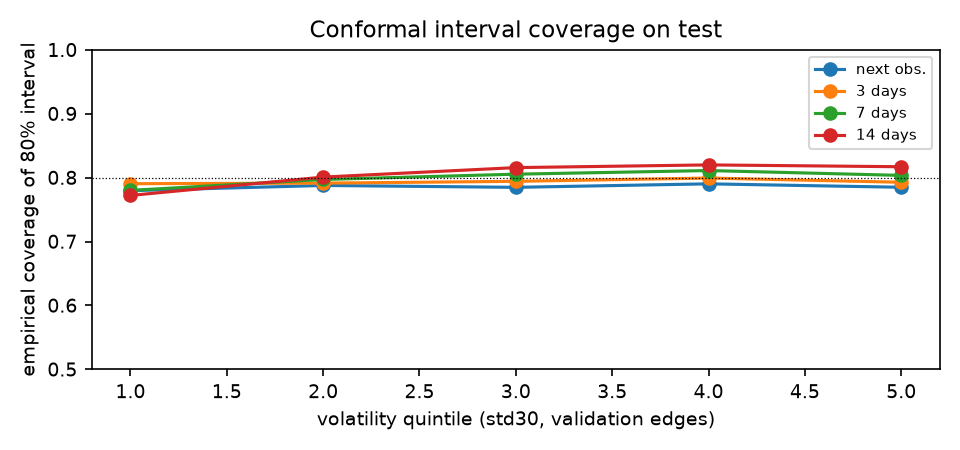
\includegraphics[width=\columnwidth]{interval_coverage.png}
\caption{Test coverage of 80\% split-conformal intervals by volatility quintile (bin edges from validation).}\label{fig:cov}
\end{figure}

\paragraph{Provenance effect.}
Measured on the mirror after the November 2025 portal change:
\begin{itemize}
  \item 80\% coverage fell to 67.6--72.9\%;
  \item relative MAE weakened to 0.993, 0.977, 0.968 and 0.944.
\end{itemize}
This had the hallmarks of a distribution shift.
Re-scoring the \emph{same frozen models} on the complete official record for the same period (Table~\ref{tab:prov}) gives:
\begin{itemize}
  \item coverage of 78.0--78.7\%, a loss of only 1.2--2.2 points against the pre-change period;
  \item relative MAE of 0.976, 0.962, 0.962 and 0.937.
\end{itemize}
The two record sets differ in which rows exist: after the change the mirror has only 62,845--97,079 test rows per horizon, against 332,275--391,425 officially.
We therefore also score both on the identical (series, origin) keys present in both (50,923--78,773 rows per horizon; last block of Table~\ref{tab:prov}).
On these identical rows, mirror coverage is 68.0--72.3\% and official coverage 78.8--79.7\%. The calibration loss is therefore not an artefact of sample composition.
Most of the apparent loss of calibration was produced by the mirror's missing reports.
Accuracy is a different matter. On official data the 7-day relative MAE still rises from 0.938 before the change to 0.962 after, so the gain over persistence shrinks from 6.2\% to 3.8\%. Part of the accuracy shift is real.
The mechanism is consistent with Section~\ref{sec:data}: three-times-longer gaps make ``next'' targets more distant and trailing windows sparser, so realised changes exceed what validation residuals calibrated on denser series anticipate.
A provenance audit is therefore a precondition for any claim about drift in this data.

\begin{table}[!t]\centering\small
\caption{Frozen models after the November 2025 portal change (2025-11-01 to 2026-04-20): mirror versus complete official record.}\label{tab:prov}
\begin{tabular}{@{}lrrrr@{}}\toprule
 & next & 3 d & 7 d & 14 d\\\midrule
Rel.\ MAE, mirror & 0.993 & 0.977 & 0.968 & 0.944\\
Rel.\ MAE, official & 0.976 & 0.962 & 0.962 & 0.937\\
80\% coverage, mirror & 67.6\% & 71.3\% & 72.0\% & 72.9\%\\
80\% coverage, official & 78.0\% & 78.7\% & 78.7\% & 78.5\%\\\midrule
\multicolumn{5}{@{}l}{\emph{Identical (series, origin) keys}}\\
Rel.\ MAE, mirror & 0.998 & 0.983 & 0.971 & 0.942\\
Rel.\ MAE, official & 0.972 & 0.958 & 0.959 & 0.930\\
80\% coverage, mirror & 68.0\% & 71.6\% & 71.9\% & 72.3\%\\
80\% coverage, official & 78.8\% & 79.7\% & 79.7\% & 79.3\%\\\bottomrule
\end{tabular}\end{table}
